	\begin{figure}[!thpb]
		\centering
		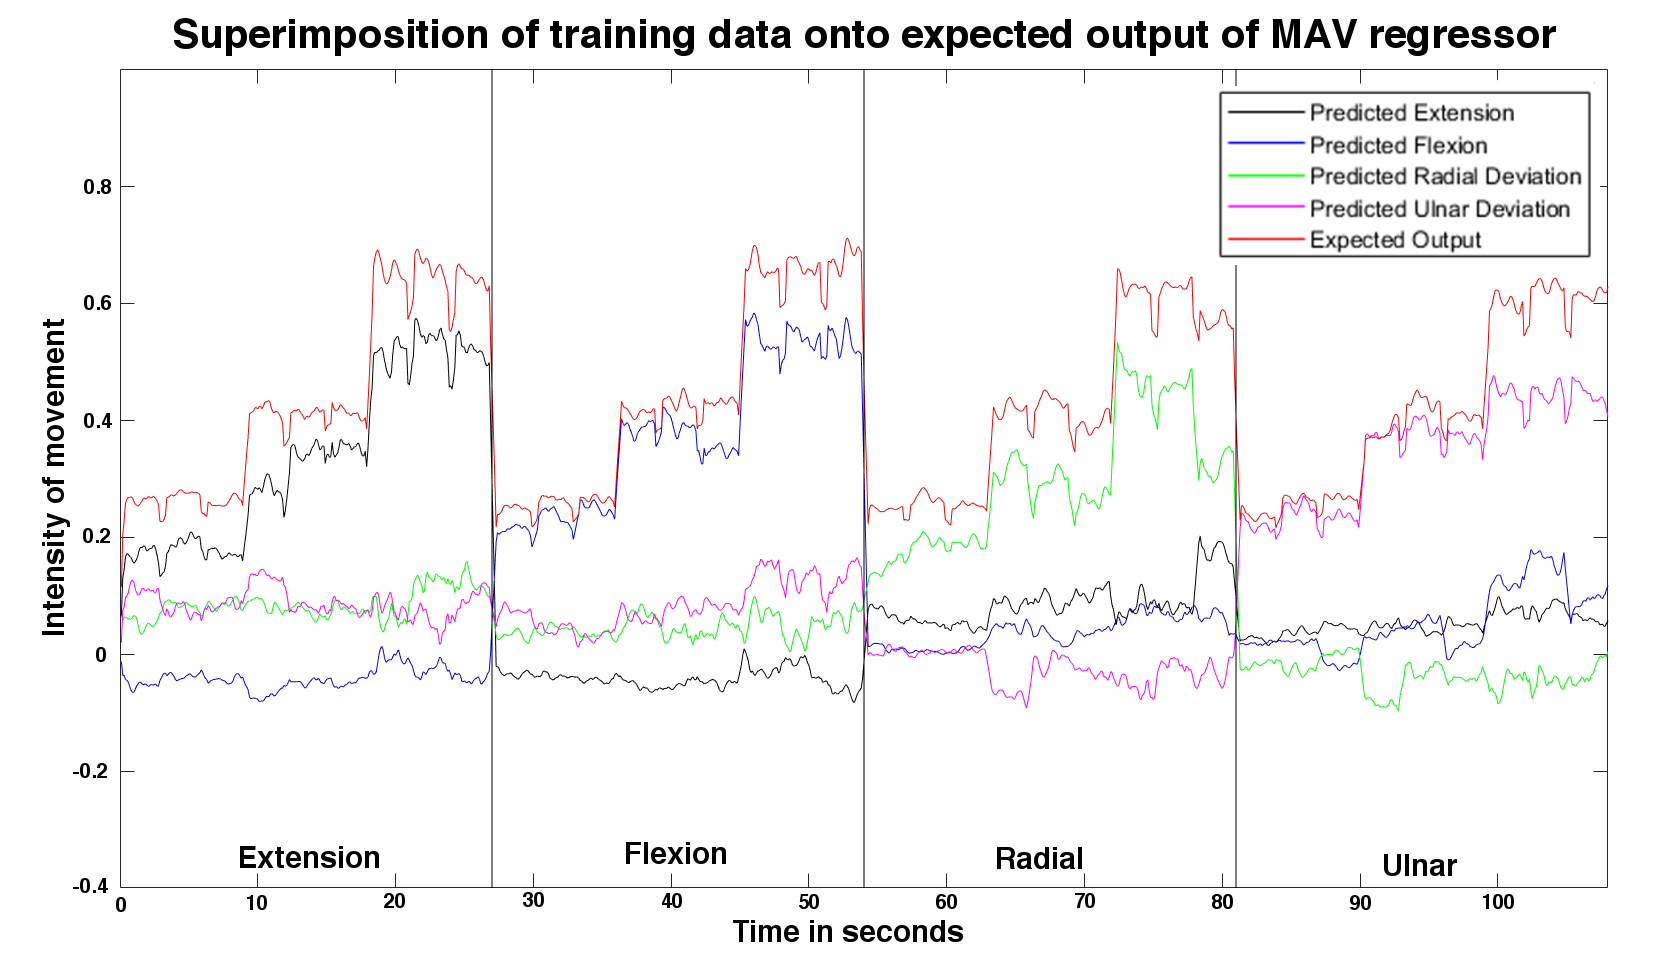
\includegraphics[width=0.4\textwidth]{figures/NewSuperPositionTestDataMAV}  %<--but is not needed.
		\caption{Plot of the actual data, red plot, superimposed on the output of the regressors trained with the MAV features. The plot is divided into four segments, where each segment shows a different movement performed. Each segment has the same sample size.}
		\label{fig:SuperPositionTrainingMAV}  %<--give the figure a label, so you can reference!
	\end{figure}
	
	\begin{figure}[!thpb]
		\centering
		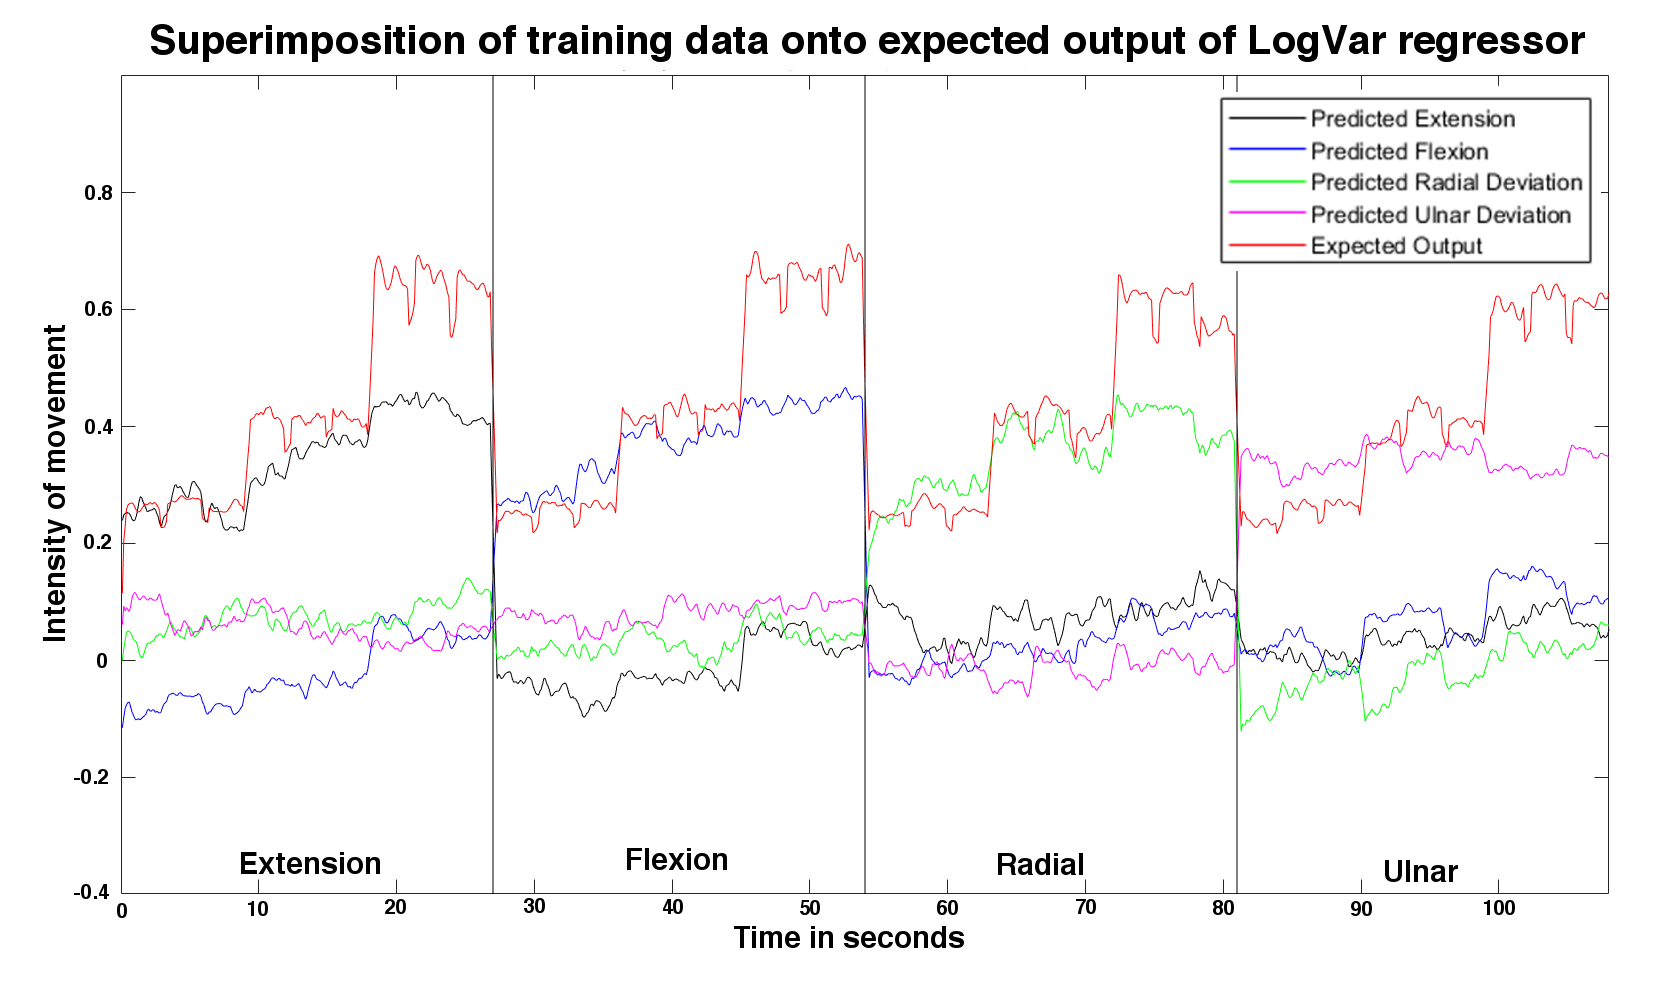
\includegraphics[width=0.4\textwidth]{figures/NewSuperPositionTestDataLogVar}  %<--but is not needed.
		\caption{Plot of the actual data, red plot, superimposed on the output of the regressors trained with the LogVar features. The plot is divided into four segments, where each segment shows a different movement performed. Each segment has the same sample size.}
		\label{fig:SuperPositionTrainingLogVar}  %<--give the figure a label, so you can reference!
	\end{figure}
	
	\begin{table}[!thpb]
		\begin{center}
			\begin{tabular}{l l l}
				\hline
				\textbf{Feature} & \textbf{Overall mean error} & \textbf{Standard deviation}\\
				\hline
				Extension & 0.1030 & $\pm 0.0210$ \\
				Flexion & 0.1102 & $\pm 0.0296$ \\
				Radial Deviation & 0.1206 & $\pm 0.0298$ \\
				Ulnar Deviation & 0.1143 & $\pm 0.0334$ \\
				Overall & 0.1059 & $\pm 0.0306$ \\
				\hline
			\end{tabular}
			\caption{RMSE for the implemented MAV regressor}
		\end{center}
	\end{table}
	
	\begin{table}[!thpb]
		\begin{center}
			\begin{tabular}{l l l}
				\hline
				\textbf{Feature} & \textbf{Overall mean error} & \textbf{Standard deviation}\\
				\hline
				Extension & 0.1157 & $\pm 0.0469$ \\
				Flexion & 0.1102 & $\pm 0.0241$ \\
				Radial Deviation & 0.1142 & $\pm 0.0256$ \\
				Ulnar Deviation & 0.1312 & $\pm 0.0310$ \\
				Overall & 0.1178 & $\pm 0.0272$ \\
				\hline
			\end{tabular}
			\caption{RMSE for the implemented LogVar regressor}
		\end{center}
	\end{table}
	
	Analysing the RMSE of the regression models' response to the training data, it was found that there's a significant difference (p = 0.0044) between MAV and LogVar, where it was shown that LogVar (mean = 0.1178, std = 0.0272) has a higher mean than MAV (mean = 0.0159, std = 0.0306).
	
	\begin{table}[!thpb]
		\begin{center}
			\begin{tabular}{l l l}
				\hline
				\textbf{Feature} & \textbf{Overall mean error} & \textbf{Standard deviation}\\
				\hline
				Extension & 0.1646 & $\pm 0.0753$ \\
				Flexion & 0.1391 & $\pm 0.0841$ \\
				Radial Deviation & 0.2018 & $\pm 0.0424$ \\
				Ulnar Deviation & 0.1743 & $\pm 0.0905$ \\
				Overall & 0.1700 & $\pm 0.0759$ \\
				\hline
			\end{tabular}
			\caption{RMSE for the implemented MAV regressor}
		\end{center}
	\end{table}
	
	
	\begin{table}[!thpb]
		\begin{center}
			\begin{tabular}{l l l}
				\hline
				\textbf{Feature} & \textbf{Overall mean error} & \textbf{Standard deviation}\\
				\hline
				Extension & 0.1552 & $\pm 0.0514$ \\
				Flexion & 0.1680 & $\pm 0.0508$ \\
				Radial Deviation & 0.1681 & $\pm 0.0540$ \\
				Ulnar Deviation & 0.2078 & $\pm 0.0621$ \\
				Overall & 0.1748 & $\pm 0.0563$ \\
				\hline
			\end{tabular}
			\caption{RMSE for the implemented LogVar regressor}
		\end{center}
	\end{table}
	
	\begin{table}[!thpb]
		\begin{center}
			\begin{tabular}{l l}
				\hline
				\textbf{Compared features} & \textbf{P-Value}\\
				\hline
				LogVar, MAV & 0.0044 \\
				LogVar test data, MAV test data & 0.1138 \\
				LogVar test data, LogVar & 0.0001 \\
				MAV test data, MAV & 0.000002 \\
				\hline
			\end{tabular}
			\caption{P-Values for comparison of the features}
		\end{center}
	\end{table}
	
	It was found that there is a significant difference (p = 0.0001) between the RMSE for test data (mean = 0.1748, std = 0.0563) and training data (mean = 0.1178, std = 0.0272) for LogVar. A significant difference (p = 0.000002) was also found for the test data (mean = 0.1700, std = 0.0759) and training data (mean = 0.1059, std = 0.0306) for the MAV based regression models. No significant difference (p = 0.1138) was found between MAV (mean = 0.1700, std = 0.0759) and LogVar (mean = 0.1748, std = 0.0563) regression models with test data.
	
	\begin{figure}[!thpb]
		\centering
		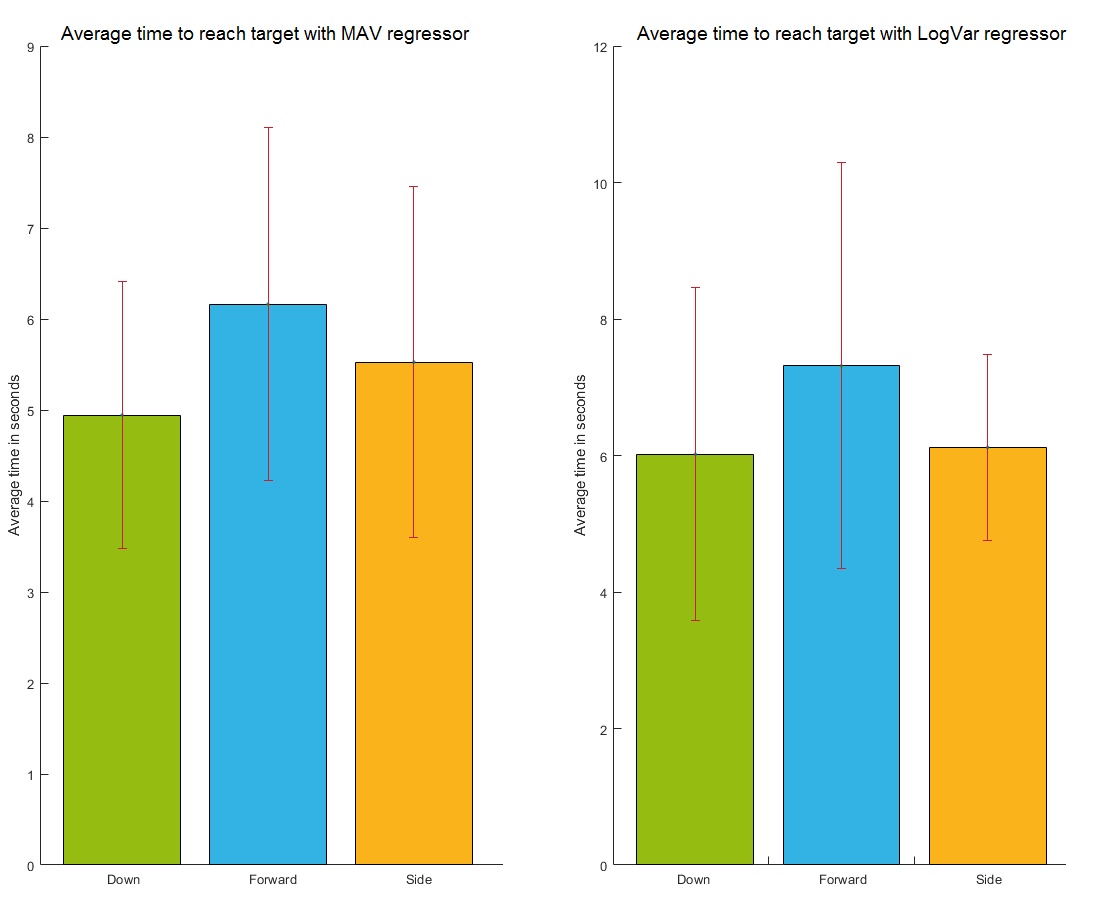
\includegraphics[width=0.4\textwidth]{figures/GotItTime}  %<--but is not needed.
		\caption{Plot of the actual data, red plot, superimposed on the output of the regressors trained with the MAV features. The plot is divided into four segments, where each segment shows a different movement performed. Each segment has the same sample size.}
		\label{fig:GotItTime}  %<--give the figure a label, so you can reference!
	\end{figure}
	
	\begin{table}![thpb]
		\begin{center}
			\begin{tabular}{l l l}
				\hline
				\textbf{Limb position, feature} & \textbf{Overall mean error} & \textbf{Standard deviation}\\
				\hline
				Down, MAV & 5.3377 & $\pm 1.5696$ \\
				Forward, MAV & 8.1791 & $\pm 4.7145$ \\
				Side, MAV & 6.0490 & $\pm 2.0490$ \\
				Down, LogVar & 6.5404 & $\pm 2.5315$ \\
				Forward, LogVar & 7.9123 & $\pm 3.4572$ \\
				Side, LogVar & 6.9325 & $\pm 2.3036$ \\
				\hline
			\end{tabular}
			\caption{Test scores for the different limb for MAV and LogVar regressors}
		\end{center}
	\end{table}
	\begin{table}[!thpb]
		\begin{center}
			\begin{tabular}{l l}
				\hline
				\textbf{Feature} & \textbf{P-Value}\\
				\hline
				MAV & 0.8948 \\
				LogVar & 0.2359 \\
				\hline
			\end{tabular}
			\caption{P-Values for comparison of the score in different limb positions with MAV and LogVar}
		\end{center}
	\end{table}
	
	When comparing the score for different limb positions, no significant difference was found for either MAV (p = 0.8948) or LogVar (p = 0.2359).
	
	\begin{table}[!thpb]
		\begin{center}
			\begin{tabular}{l l l}
				\hline
				\textbf{Limb position, feature} & \textbf{Overall mean error} & \textbf{Standard deviation}\\
				\hline
				Down, MAV & 15.5556 & $\pm 0.7265$ \\
				Forward, MAV & 15.1111 & $\pm 1.0541$ \\
				Side, MAV & 15.2222 & $\pm 0.8333$ \\
				Down, LogVar & 15.4444 & $\pm 0.7265$ \\
				Forward, LogVar & 15 & $\pm 1.8020$ \\
				Side, LogVar & 15.3333 & $\pm 1.1180$ \\
				\hline
			\end{tabular}
			\caption{Targets reached in the target test with the MAV and LogVar regressors.}
		\end{center}
	\end{table}
	
	\begin{table}[!thpb]
		\begin{center}
			\begin{tabular}{l l}
				\hline
				\textbf{Feature} & \textbf{P-Value}\\
				\hline
				MAV & 0.0212 \\
				LogVar & 0.4220 \\
				\hline
			\end{tabular}
			\caption{P-Values for comparison of the number of reached targets in different limb positions with MAV and LogVar}
		\end{center}
	\end{table}
	
	It was shown that there is a significant difference (p = 0.0212) between the number of targets reached in the different positions for MAV, where the limb pointed forward yielded worst results (mean = 15.1111, std = 1.0541). No significant difference (p = 0.4220) was found between the limb positions for LogVar.
	
	\begin{figure}[!thpb]
		\centering
		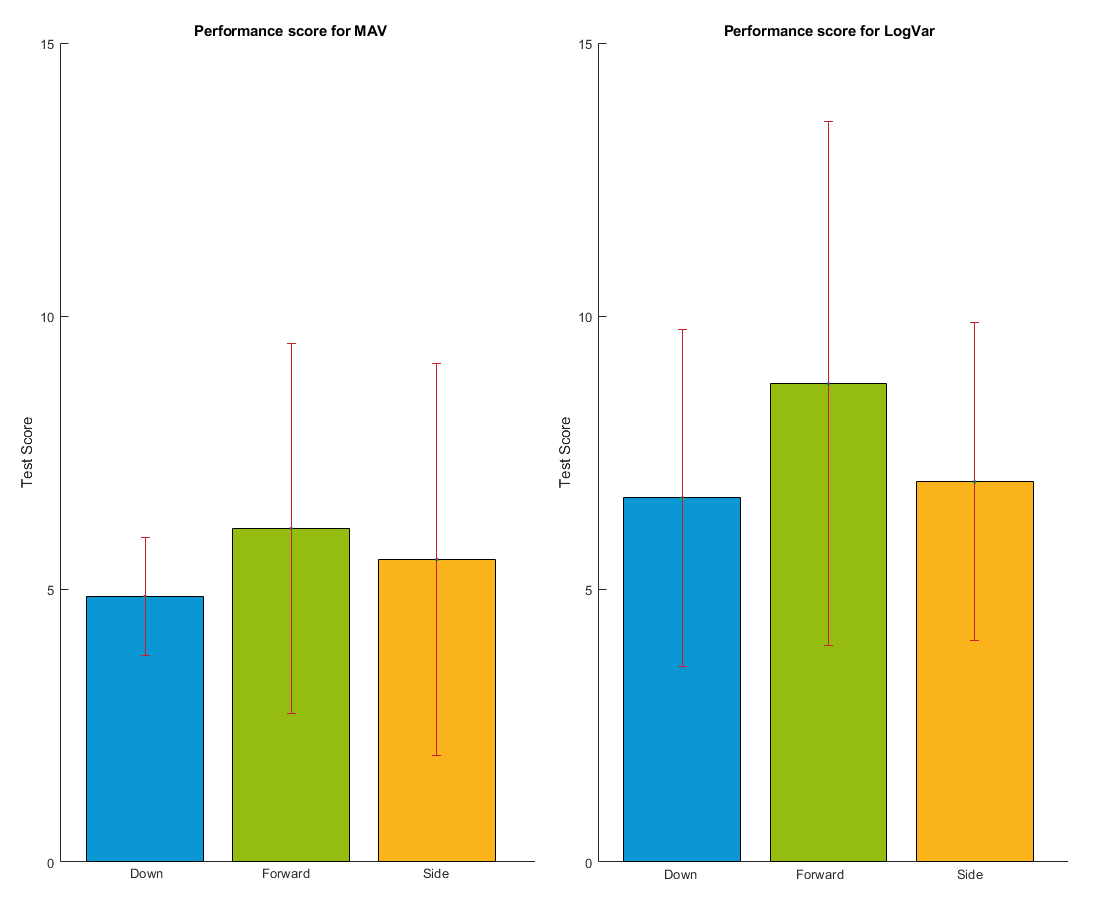
\includegraphics[width=0.4\textwidth]{figures/GotItTimeIMU}  %<--but is not needed.
		\caption{Plot of the actual data, red plot, superimposed on the output of the regressors trained with the MAV features. The plot is divided into four segments, where each segment shows a different movement performed. Each segment has the same sample size.}
		\label{fig:GotItTimeIMU}  %<--give the figure a label, so you can reference!
	\end{figure}
	
	\begin{table}[!thpb]
		\begin{center}
			\begin{tabular}{l l l}
				\hline
				\textbf{Limb position,feature} & \textbf{Overall mean error} & \textbf{Standard deviation}\\
				\hline
				Down, MAV & 4.8661 & $\pm 1.0839$ \\
				Forward, MAV & 6.1094 & $\pm 3.3852$ \\
				Side, MAV & 5.5442 & $\pm 3.5847$ \\
				Down, LogVar & 6.6691 & $\pm 3.0798$ \\
				Forward, LogVar & 8.7595 & $\pm 4.7969$ \\
				Side, LogVar & 6.9652 & $\pm 2.9144$ \\
				\hline
			\end{tabular}
			\caption{Test scores for the different limb for MAV and LogVar regressors with IMU included.}
		\end{center}
	\end{table}
	
	\begin{table}[!thpb]	
		\begin{center}
			\begin{tabular}{l l}
				\hline
				\textbf{Feature} & \textbf{P-Value}\\
				\hline
				MAV & 0.0319 \\
				LogVar & 0.4594 \\
				\hline
			\end{tabular}
			\caption{P-Values for comparison of the score in different limb positions with MAV and LogVar with IMU data included}
		\end{center}
	\end{table}
	
	A significant difference (p = 0.0319) was found between the test score in different limb positions for MAV with IMU included, where the worst performance was found with the arm pointed forward (mean = 6.1094, std = 3.3852). No significant difference (p = 0.4594) was found between limb positions for the LogVar regression model with IMU data included.
	
	\begin{table}[!thpb]
		\begin{center}
			\begin{tabular}{l l l}
				\hline
				\textbf{Limb position,feature} & \textbf{Overall mean error} & \textbf{Standard deviation}\\
				\hline
				Down, MAV & 15.8889 & $\pm 0.3333$ \\
				Forward, MAV & 15.1111 & $\pm 2.3154$ \\
				Side, MAV & 15.5556 & $\pm 1.3333$ \\
				Down, LogVar & 14.7778 & $\pm 1.7159$ \\
				Forward, LogVar & 13.5556 & $\pm 2.1858$ \\
				Side, LogVar & 14.1111 & $\pm 1.8333$ \\
				\hline
			\end{tabular}
			\caption{RMSE for the implemented LogVar regressor}
		\end{center}
	\end{table}
	
	\begin{table}[!thpb]
		\begin{center}
			\begin{tabular}{l l}
				\hline
				\textbf{Compared Features} & \textbf{P-Value}\\
				\hline
				MAV & 0.2957 \\
				LogVar & 0.0037 \\
				\hline
			\end{tabular}
			\caption{P-Values for comparison of the number of targets reached in different limb positions with MAV and LogVar with IMU data included}
		\end{center}
	\end{table}
	
	There was no significant difference found for the MAV regressor with IMU data included (p = 0.2957). The number of targets reached in different limb positions was proven significantly different (p = 0.0037) for the LogVar feature with IMU data included, where the lowest number of targets reached was found with the arm pointed forward (mean = 13.5556, std = 2.1858).
	
	\begin{figure}[!thpb]
		\centering
		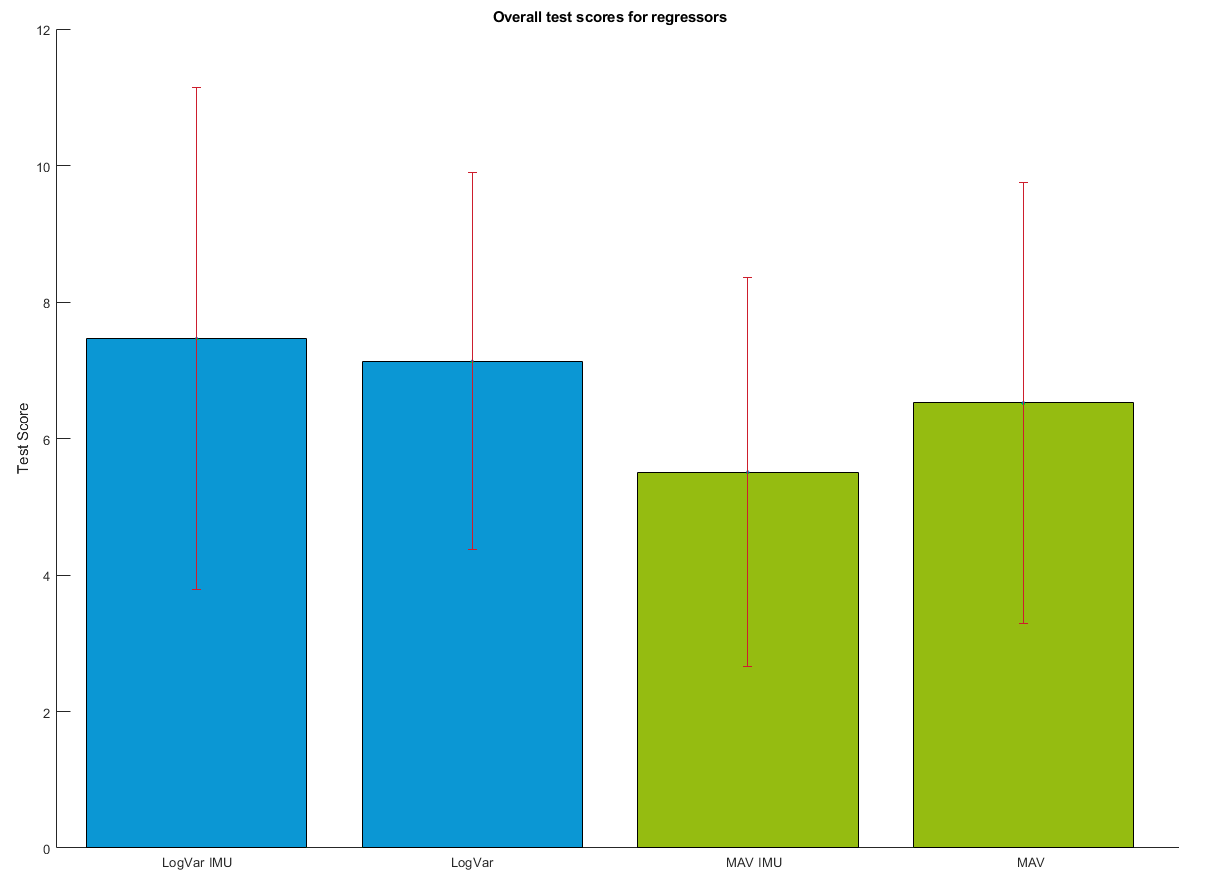
\includegraphics[width=0.4\textwidth]{figures/allRegressorBarzTimeScoreForTargetTest}  %<--but is not needed.
		\caption{Plot of the actual data, red plot, superimposed on the output of the regressors trained with the MAV features. The plot is divided into four segments, where each segment shows a different movement performed. Each segment has the same sample size.}
		\label{fig:TimeScoreTargets}  %<--give the figure a label, so you can reference!
	\end{figure}
	
	\begin{table}[!thpb]
		\begin{center}
			\begin{tabular}{l l l}
				\hline
				\textbf{Feature} & \textbf{Mean score} & \textbf{Standard deviation}\\
				\hline
				MAV & 6.5219 & $\pm 3.2253$ \\
				MAV w. IMU & 5.5066 & $\pm 2.8477$ \\
				LogVar & 7.1284 & $\pm 2.7619$ \\
				LogVar w. IMU & 7.4646 & $\pm 3.6740$ \\
				\hline
			\end{tabular}
			\caption{Average score of the target test for the four regressor designs}
		\end{center}
	\end{table}
	
	\begin{table}[!thpb]
		\begin{center}
			\begin{tabular}{l l}
				\hline
				\textbf{Compared features} & \textbf{P-Value}\\
				\hline
				LogVar w/ IMU, MAV w/ IMU & 0.5637 \\
				LogVar, MAV & 0.0833 \\
				LogVar w/ IMU, LogVar & 0.5637 \\
				MAV w/ IMU, MAV & 0.1779 \\
				\hline
			\end{tabular}
			\caption{P-Values for comparison of the overall scores of the target tests}
		\end{center}
	\end{table}
	
	A significant difference (p = 0.5637) could not be proven between the scores of the target test for LogVar with IMU data and MAV with IMU data. There was no significant difference (p = 0.0833) between the score of LogVar without IMU data and MAV without IMU data. It was also found that there is no significant difference between regression models with and without IMU data for both MAV (p = 0.1179) and LogVar (p = 0.5637).
	
	\begin{figure}[!thpb]
		\centering
		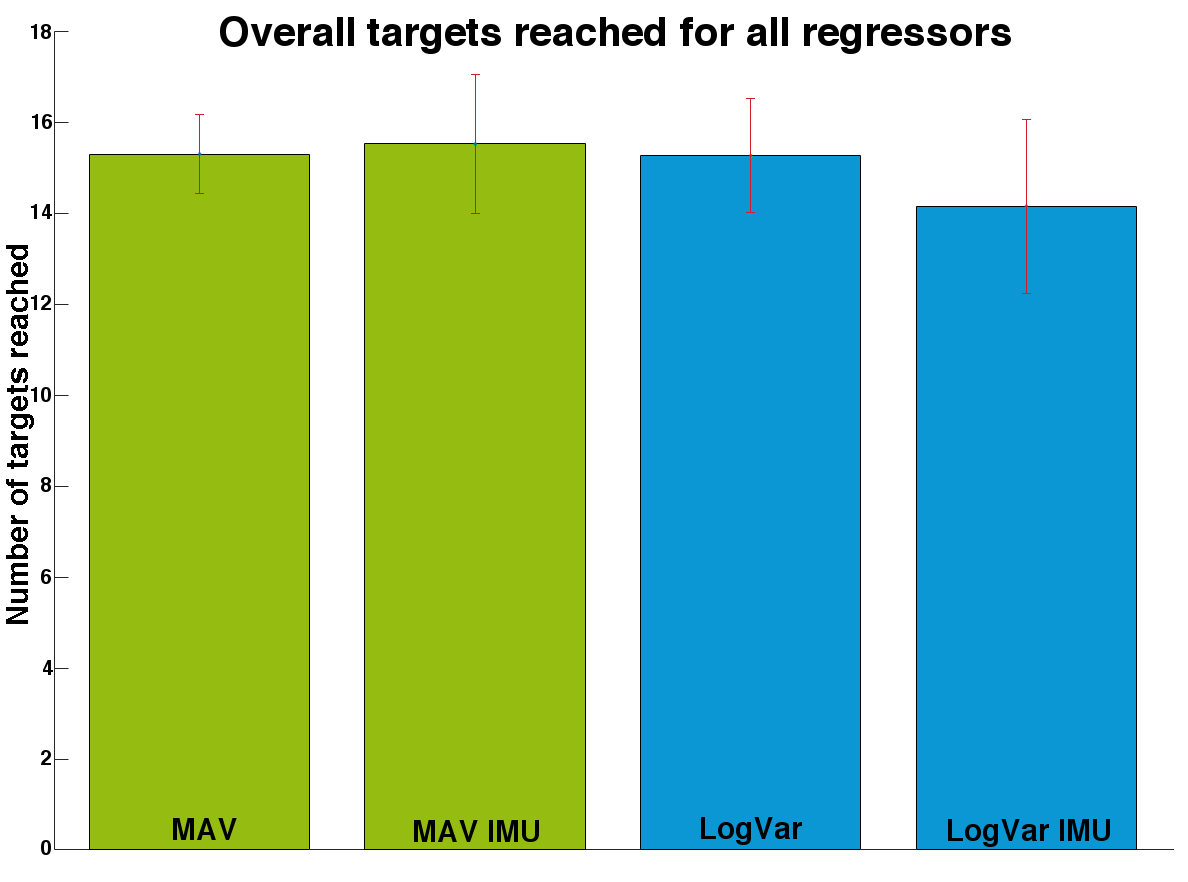
\includegraphics[width=0.4\textwidth]{figures/sumMoreBarsWithTargetsReachedForAllRegressors}  %<--but is not needed.
		\caption{Plot of the actual data, red plot, superimposed on the output of the regressors trained with the MAV features. The plot is divided into four segments, where each segment shows a different movement performed. Each segment has the same sample size.}
		\label{fig:TargetScoresTargets}  %<--give the figure a label, so you can reference!
	\end{figure}	
	
	\begin{table}[!thpb]
		\begin{center}
			\begin{tabular}{l l l}
				\hline
				\textbf{Feature} & \textbf{Overall mean error} & \textbf{Standard deviation}\\
				\hline
				MAV & 15.2963 & $\pm 0.8689$ \\
				MAV w/ IMU & 15.5185 & $\pm 1.5285$ \\
				LogVar & 15.2593 & $\pm 1.2586$ \\
				LogVar w/ IMU & 14.1481 & $\pm 1.9156$ \\
				\hline
			\end{tabular}
			\caption{Average number of targets reached in the target test for the four regressor designs}
		\end{center}
	\end{table}
	
	\begin{table}[!thpb]
		\begin{center}
			\begin{tabular}{l l}
				\hline
				\textbf{Compared Features} & \textbf{P-Value}\\
				\hline
				LogVar w/ IMU, MAV w/ IMU & 0.0017 \\
				LogVar, MAV & 1 \\
				LogVar w/ IMU, LogVar & 0.0016 \\
				MAV w/ IMU, MAV & 0.0124 \\
				\hline
			\end{tabular}
			\caption{P-Values for comparison targets reached in the target tests}
		\end{center}
	\end{table}
	
	A significant difference (p = 0.0017) was found between targets reached when IMU was included, where LogVar (mean = 14.1481, std = 1.9156) was proven worse than MAV (mean = 15.5185, std = 1.5285). There was a significant difference (p = 0.0016) between LogVar with (mean = 14.1481, std = 1.9156) and without (mean = 15.2593, std = 1.2586) IMU data. The same significant difference (p = 0.0124) between MAV with (mean = 15.5185, std = 1.5285) and without (mean = 15.2963, std = 0.8689) IMU data. There was no difference (p = 1) between targets reached with LogVar and MAV when IMU was not included.
	
	
	%	\subsection{Separability of the data} 
	
	
	
	%PCA performance for both features extracted is illustrated in Fig. \ref{PCA_MVA} (MVA) and in Fig. \ref{PCA_logvar} (logarithmic variance).
	%The importance of each component for MAV and logarithmic variance is represented in Fig. \ref{PCA_MVA}(a) and Fig. \ref{PCA_logvar}(a) respectively. On the one hand for the MAV feature making use of the three first components, 93.8\% of the data set can be described. On the other hand for the logarithmic variance feature the 93.97\% of the data set is describe with the three first components. This three PC have been plot for both features Fig. \ref{PCA_MVA}(b) and Fig. \ref{PCA_logvar}(b). There is no presence of remarkable outliers on two data sets and the formed clusters are easily distinguishable.
	
	
	%	\subsection{Regression accuracy} 
	
	%Through a quantitative examination of the figure(figure),is observed that MAV performed slightly better than the logarithmic variance for low intensities. However, both estimates yielded inaccurate fitting in high intensities, especially for ulnar deviation of the wrist. It has been extracted from the results illustrated in (figure), which represent the RMSE of the four different regressos for both features of the training data, than $RMSE_{MAV}$= 0.0867$\pm 0.031$ and $RMSE_{logvar}$= 0.1047$\pm 0.0273$. Overall MAV provided a lower mean but a higher standard deviation compared with logarithmic variance.
	
	%\begin{figure}[thpb]
	%\centering
	%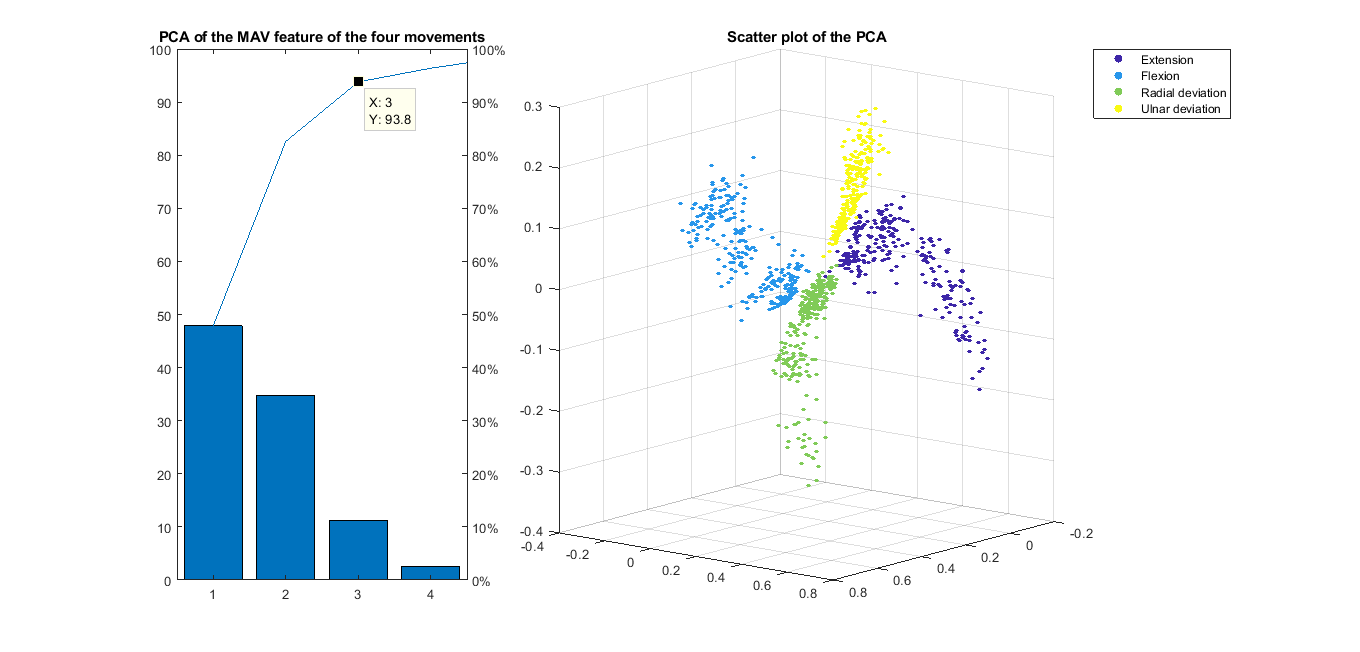
\includegraphics[scale=.27]{Figures/pcasubplotMAV}
	%\caption{Inductance of oscillation winding on amorphous
	%	magnetic core versus DC bias magnetic field}
	%\label{PCA_MVA}
	%\end{figure}
	
